% !TEX TS-program = pdflatex
% !TEX encoding = UTF-8 Unicode

% This is a simple template for a LaTeX document using the "article" class.
% See "book", "report", "letter" for other types of document.

\documentclass[11pt]{article} % use larger type; default would be 10pt

\usepackage[utf8]{inputenc} % set input encoding (not needed with XeLaTeX)

%%% Examples of Article customizations
% These packages are optional, depending whether you want the features they provide.
% See the LaTeX Companion or other references for full information.

%%% PAGE DIMENSIONS
\usepackage{geometry} % to change the page dimensions
\geometry{a4paper} % or letterpaper (US) or a5paper or....
% \geometry{margin=2in} % for example, change the margins to 2 inches all round
% \geometry{landscape} % set up the page for landscape
%   read geometry.pdf for detailed page layout information

\usepackage{graphicx} % support the \includegraphics command and options

% \usepackage[parfill]{parskip} % Activate to begin paragraphs with an empty line rather than an indent

%%% PACKAGES
\usepackage{booktabs} % for much better looking tables
\usepackage{array} % for better arrays (eg matrices) in maths
\usepackage{paralist} % very flexible & customisable lists (eg. enumerate/itemize, etc.)
\usepackage{verbatim} % adds environment for commenting out blocks of text & for better verbatim
\usepackage{subfig} % make it possible to include more than one captioned figure/table in a single float
\usepackage{hyperref}
\hypersetup{colorlinks=true,linkcolor=black,filecolor=magenta,urlcolor=cyan}
\usepackage{titling}
\usepackage{atbegshi}
\AtBeginDocument{\AtBeginShipoutNext{\AtBeginShipoutDiscard}}
\usepackage{amsmath}
\usepackage{float}
% These packages are all incorporated in the memoir class to one degree or another...

%%% HEADERS & FOOTERS
\usepackage{fancyhdr} % This should be set AFTER setting up the page geometry
\pagestyle{fancy} % options: empty , plain , fancy
\renewcommand{\headrulewidth}{0pt} % customise the layout...
\lhead{}\chead{}\rhead{}
\lfoot{}\cfoot{\thepage}\rfoot{}

%%% SECTION TITLE APPEARANCE
\usepackage{sectsty}
\allsectionsfont{\sffamily\mdseries\upshape} % (See the fntguide.pdf for font help)
% (This matches ConTeXt defaults)

%%% ToC (table of contents) APPEARANCE
\usepackage[nottoc,notlof,notlot]{tocbibind} % Put the bibliography in the ToC
\usepackage[titles,subfigure]{tocloft} % Alter the style of the Table of Contents
\renewcommand{\cftsecfont}{\rmfamily\mdseries\upshape}
\renewcommand{\cftsecpagefont}{\rmfamily\mdseries\upshape} % No bold!

%%% END Article customizations

%%% The "real" document content comes below...

\pretitle{\begin{center}\fontsize{34bp}{34bp}\selectfont}
	\posttitle{\vspace{14bp}\par\includegraphics[width=350pt]{Figures/"0) Title"/Title-image-01.png}\par\end{center}}
\preauthor{\begin{center}\fontsize{18bp}{18bp}\selectfont}
	\postauthor{\par\end{center}}
\predate{\begin{center}}
	\postdate{\par\end{center}}

\title{sptPALM Analysis Guide}
\author{Adam Hines}
\date{}

\begin{document}

\begin{center}{\maketitle{\LARGE{A simplified particle localisation and tracking solution.}}}
\end{center}

%%% Table of Contents Section %%%%
\newpage
\tableofcontents

\newpage

\section{Introduction}

Thank you for downloading and trying sptPALM Analysis (SPA). SPA is a semi-automated single particle tracking tool utilising a graphical user interface (GUI) that interfaces with the ImageJ plugin TrackMate. Users are able to automatically load image sequences of photoactivatable localisation microscopy (PALM) and utilise a built in tracking algorithm for single particles (spt). The semi-automated component refers to the fact that users are required to convert image sequences to the correct format and determine threshold values for spot detection themselves. This is advantageous as auto-detecting threshold values can often lead to over or under-estimation of the spot detection threshold. \\
SPA was developed by Adam Hines at the Queensland Brain Institute. If utilising this tool in your publications, please cite (\textit{reference}) as well as the original author of TrackMate (\textit{reference}).

\subsection{Overview}

This chapter will provide an overview on how the analysis script operates and what algorithms the program uses in order to reliably detect and track the mobility of particles. It will begin by briefly describing the spot detection component of the analysis and the tracking algorithm utilised, however for further information please refer to the source documentation of TrackMate (\href{https://imagej.net/TrackMate_Algorithms}{TrackMate Algorithms}).

\subsection{Spot detection}

The chosen method for spot detection was the Lapacian of Gaussian (LoG) fitting algorithm. This algorithm takes low resolution spots and fits a LoG over pixels in an x,y plane. The threshold specified will determine which detected spots are appropriate and which are not, and this should be done by the user with their own eyes as this avoids having too many innappropriate or too few appropriate spots. A visualisation of how the spot detection algorithm works is presented in Figure 1.\\

There are also two settings that are enabled during the spot detection component of SPA. Median filtering and subpixel localisation are enabled to remove the generation of 'jagged' particle linked tracks as well as to improve the acuity of spot detection.\\

There are other methods for spot detection available in TrackMate, and it should be encouraged to explore the best option for your needs. Embedded into the software however is the LoG detection. SPA is an open-sourced program, so editing the source code will be your only option in order to hardwire a difference detection algorithm - and the same goes for the tracking method (covered in the next section).

	\begin{figure}[H]
	\center{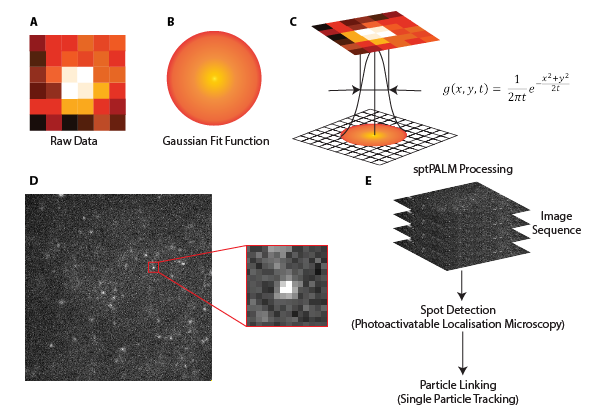
\includegraphics[width=\textwidth]{Figures/"1) Introduction"/PALM-01.png}}
	\caption{Visualisation of particle detection in SPA. \textbf{A} Schematic of typical raw data observed in photoactivatable light microscopy (PALM) 					experiments, consisting of low resolution pixels with a bright centre with decreasing intensity from the centre. \textbf{B} Example of a Gaussian fit of the raw 		data in \textbf{A}. \textbf{C} The Gaussian fit function transposing the low resolution raw data into a high-resolution spot. Formula shown if the Lapacian of 		Gaussian (LoG) spot detection used in SPA analysis. \textbf{D} Representative raw data from a PALM experiment highlighting a single spot. \textbf{E} 				Schematic of the workflow used in SPA. Image sequences have parallel threading in spot detection and particle linking in subsequent tracking stages of 			analysis.}
	\end{figure}

\subsection{Particle linking}

Single particle tracking has remained a problem for researchers for a very long time. Reliable tracking of multiple particles over a long time frame can cause issues such as linking particles together that are not the same, incorrectly linking a particle that has newly appeared, or even incorrectly ending a track. Figure 2 \textbf{A} shows an example of what a tracked particle looks like in an x,y plane. SPA uses the particle linking algorithm known as a linear assignment problem (LAP) cost matrix in order to evaluate and ultimately minimise the cost in favour of the most likely linked particles between frame  $t_1$ and $t_2$. The cost values in this context is simply the squared displacement ($\delta^2$) between two detected particles. Each particle in frame $n_1$ has a potential link associated to every particle in frame $t_2$ (Figure 2 \textbf{B}), meaning that for each particle in $t_1$ there are several cost values associated to that particle and the LAP algorithm attempts to find the lowest sum cost for every single particle between frames $t_1$ and $t_2$. \\

What about particles that have no prior or future link? At a certain point during a recording, particles will bleach and new particles will appear, so how are these dealt with? A separate matrix is established where the previous cost value of a particle linking, ($\delta^2$), is multiplied by a factor of 1.05. If there is a cost that is lower than this value, the particle will have a potential link. If the multiplied cost factor satisfies the lowest sum calculation then that particle, depending on context, will either have no future linkages or is defined as a newly appearing particle. \\

Particles that are at disparate ends of an x,y plane are easily dealt with by simply setting a maximum cutoff that two particles can physically link. If the ($\delta^2$) exceeds this value, then the link is impossible and cannot satisfy the lowest cost sum. A summary of the potential outcomes of a particle linking between two frames is shown in Figure 2 \textbf{C}.

	\begin{figure}[H]
	\center{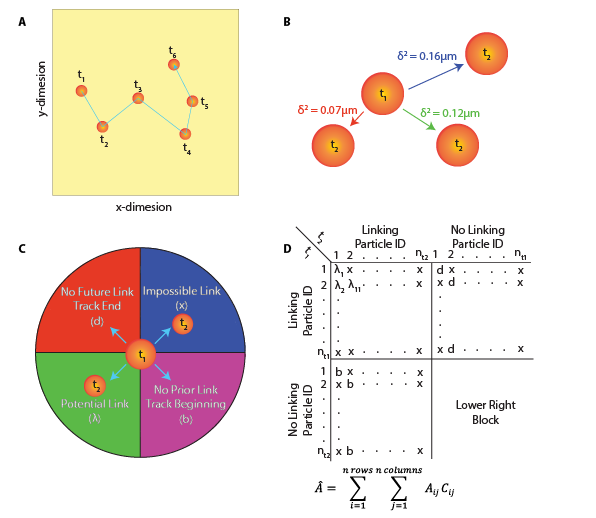
\includegraphics[width=\textwidth]{Figures/"1) Introduction"/SPT-01.png}}
	\caption{Use of a Linear Assignment Problem (LAP) Cost Matrix to Link Particles Between Frames. \textbf{A} Schematic of how a particles trajectory through 		time in an x,y plane may look, $t_n$ refers to the time or frame number. \textbf{B} A particle in $t_1$ will have multiple potential linking particles in $t_2$, 			with an associated cost value $\delta^2$. \textbf{C} The possible outcomes for a particle in $t_2$ following $t_1$. \textbf{D} Schematic of the cost matrix 			utilised in the LAP. To satisfy the LAP, the sum of the cost is minimised as low as possible.}
	\end{figure}

\subsection{Mean squared displacement and diffusion coefficients}

The main metric utilised in single particle tracking is the mean squared displacment (MSD), which describes the distance a particle moves from its initial displacement in relation to time. In association with the MSD, the diffusion coefficient is another metric that describes the diffusivity of molecules in space. The diffusion coefficient is empirically derived from the MSD and combined describe the mobility of tracked particles (Figure 3 \textbf{A} and \textbf{B}). The diffusion coefficient values can be represented on a curve as a relative frequency of a whole, taking a logarithmic conversion and counting the frequency in bins of -5 to 1.\\


Useful quantifications of the MSD and diffusion coefficients are the area under the curve and the mobile to immobile ratio, defined as the ratio between binned log diffusion coefficients above -1.6 (related to a speed of X) and below -1.6 (Figure 3 \textbf{C} and \textbf{D}). These two metrics allow for simple statistical analysis.\\

SPA automatically calculates the MSD and diffusion coefficients thanks to a piece of code from \textit{Reference}. Area under the curve and mobile to immobile ratios are not currently calculated within SPA. 

	\begin{figure}[H]
	\center{\includegraphics[width=\textwidth]{Figures/"1) Introduction"/sptMetrics-01.png}}
	\caption{Example of the metrics of single particle tracking experiments. \textbf{A} Relative frequency of diffusion cofficients in Munc18-1 mEos2 tracked 			particles transfected in PC12 cells stimulated with $BaCl_2$ in the presence of dimethyl sulfoxide (DMSO) or $3\mu M$ propofol. \textbf{B} Mean square displacment of mEos2 particles tracked over time. \textbf{C} Mobile to immobile ratio calculated from the diffusion coefficients in \textbf{A} and area under the curve calculated from \textbf{B}.}
	\end{figure}

\subsection{Comparison of SPA to MetaMorph/PALMTracer}

How does SPA stack up against other localisation and tracking software? Given that TrackMate is a completely open-sourced and free plugin that also happens to run in an open-source and free software, Fiji, how would it fare against MetaMorph - a several thousand dollar piece of software that is often unaccessible to a lot of researchers. MetaMorph makes use of a plugin called PALMTracer, developed by John-Baptiste (\textit{Reference}), in order to localise and track particles. PALMTracer is not an automated workflow and requires the user to manually process each image sequence themselves, in comaprison to SPA which allows users to click a single button and walk away.\\

We can clearly see in Figure 4 that there is no significant difference between analysis performed on MetaMorph vs SPA/TrackMate. 

	\begin{figure}[H]
	\center{\includegraphics[width=\textwidth]{Figures/"1) Introduction"/MetaMorphTrackMate.png}}
	\end{figure}

\section{Using SPA}

This section will explore how to setup, run, and look at the output of SPA. In order to run SPA, you will require MATLAB 2017b or higher as well as some considerable computing power. SPA will run on most modern computers, however older machines may struggle to allocate appropriate computing power for analysis, particularly for large image sequences (1gb). There is a copy of Fiji included with the download and is stored locally in the analysis folders.

\subsection{Installing and setting up SPA}

To begin, obtain the latest version of SPA through GitHub. Create a GitHub account and download the code and store it somewhere local on your computer (e.g. the MATLAB directory). Access the SPA GitHub repositry \href{https://github.com/AdamDHines/sptPALM-Analysis.git}{here}, click "Clone or download", and then "Download ZIP" (Figure 5).

	\begin{figure}[H]
	\center{\includegraphics[width=\textwidth]{Figures/"2) Using SPA"/DownloadGit.jpg}}
	\caption{Accessing GitHub to download the latest version of SPA.}
	\end{figure} 

Once the ZIP folder has been downloaded, create a folder such as "sptPALM" in a local directory (e.g. the MATLAB folder in Documents) and open MATLAB. Once open, you must set the current directory of MATLAB to the folder that you created that contains all of the code and the "start.m" file. To do so, click the folder icon with the green arrow just above the Current Folder panel on the left hand side (Figure 6).

	\begin{figure}[H]
	\center{\includegraphics[width=\textwidth]{Figures/"2) Using SPA"/ChangeDir-01.jpg}}
	\caption{Changing the current working directory to the SPA analysis folder.}
	\end{figure}

Once this is complete, your Current Folder in MATLAB will look something like this (Figure 6). \\ 

Now we can go ahead and run SPA. In the command window of MATLAB, type "start" and hit enter. This will initialise the \textit{start.m} script and launch the graphical user interface. When a fresh install of SPA is performed, you will need to set a default directory to search for files. This can be done by simply pressing "Set directory" in the File directory panel up the top or by going File - Set File Directory (Figure 7). Once this is done, the default directory will be saved and you won't have to set it again. \\

Congratulations, SPA is now setup on your machine. The next few sections will detail how data files should be prepared and organised in order for the analysis to work.

	\begin{figure}[H]
	\center{\includegraphics[width=\textwidth]{Figures/"2) Using SPA"/SPACurDir-01.jpg}}
	\caption{Current directory with SPA code.}
	\end{figure}

	\begin{figure}[H]
	\center{\includegraphics[width=\textwidth]{Figures/"2) Using SPA"/DefDirSet-01.jpg}}
	\caption{Setting the default working directory in SPA.}
	\end{figure}

\subsection{Preparation of image sequences}

The image sequences that are used in SPA are .tif stacks. Any other file will not be recognised by SPA and won't be able to be utilised in analysis. Therefore, it is necessary to convert any image sequences to .tif using ImageJ. It is highly recommended that when exporting image sequences from the imaging software of your choice, that you save it in the native format in order to retain metadata about the recordings and then convert to .tif afterwards. What we will also do during this time is establish our threshold values for the spot detection component of the analysis.\\

To begin, open your image sequence in ImageJ. Check the sequence that the properties are correct, i.e. that the calibration settings for pixel height and width have been set and that the sequence is in terms of t and not z (analysis will stall if the t and z are swapped). Also ensure that the unit of length is "micron". Change the settings if necessary and hit 'OK' (Figure 8). In general, if you're loading the sequence from the source file containing the metadata ImageJ will automatically alter the properties to match.\\

	\begin{figure}[H]
	\center{\includegraphics[width=\textwidth]{Figures/"2) Using SPA"/PropertiesSet-01.jpg}}
	\caption{Checking the image sequence properties for calibration and correct z and t orientation.}
	\end{figure}
	
We now want to determine the threshold value, as well as the spot diameter, for the localisation component of the analysis. Open TrackMate by clicking Plugins $\rightarrow$ Tracking $\rightarrow$ TrackMate. The TrackMate GUI will open and simply click next until you reach the 'LoG Detector' settings panel. Here, determine the appropriate spot diameter and threshold value for the recording. \textit{\textbf{Important}} Ensure that both median filtering and subpixel localisation are selected. Use the preview button to view how the settings localise spots. Make note of the diamaeter and the threshold value for each individual movie, we will tell SPA when we come to analyse the files what these are.

	\begin{figure}[H]
	\center{\includegraphics[width=\textwidth]{Figures/"2) Using SPA"/TrackMateSpot-01.jpg}}
	\caption{Setting the spot diameter and threshold value for image sequences.}
	\end{figure}

Once that's done, all we need to do now is save the sequence as .tif by going to File $\rightarrow$ Save as... $\rightarrow$ Tiff... The next section will show you how to organise your data structures such that the analysis script can search for and find the files for analysis.

\subsection{File directory structure}

The file structure for the image sequences is very crucial and must be followed exactly. If it is not follow correctly, then the analysis script will not load or find any sequences to analyse and will just throw an error. In short, the sequences are all organised into individual folders inside of a parent folder. An example of this would be a parent folder of \textit{Sx1a-mEos2 28-03-2019} and within this folder are several sub-folders \textit{Recording 1, recording 2, recording 3, etc.}. The sub-folders are where the original recording (the one containing meta-data) and the .tif converted file should be stored. Adjusting to this file structure from the beginning from saving the initial recordings will save a lot of time in the future.\\

Let's have a look at what this file structure is. From left to right, we have the main data folder where we can see the folder \textit{20190320} - the folder that contains the sub-folders with our recordings in them. In the middle, we see all of the sub-folders of individual recordings, and on the right we have the contents of the sub-folder. Notice the raw \textit{.czi} file and the converted .tif that has been made. SPA will search through all of the folders and try to find a .tif file, and eliminate everything else. This is why it's so important to convert all of the image sequences into .tif before continuing. If a .tif is missing from the folder, the analysis will still run but skip over that experiment.

	\begin{figure}[H]
	\center{\includegraphics[width=\textwidth]{Figures/"2) Using SPA"/FolderStruct-01.jpg}}
	\caption{Folder directory structure for the analysis of files.}
	\end{figure}

SPA will output all of the analysis into the same parent folder as the analysis, so getting used to this structure early on will be of great benefit to using the software. The next section will focus on how to set the analysis parameters (but not how to derive them to tailor your experiments).

\subsection{Setting analysis parameters}

\subsection{Setting threshold values}

\subsection{Running analysis and analysing results}

\end{document}
